
\newcommand{\submitpaper}{}

\newcommand{\completepaper}{}

\newcommand{\cappedpaper}{}

%%\newcommand{\verbosepaper}{}


%%%%%%%%%%%%%%%%%%%%%%%%%%%%%%%%%%%%%%%%%%%%%%%%%%%%%%%%%%%%%%%%%%%%%%
%
%  Epigenetic Robotics 2003
%
%  We are using SAB format.
%  Choose 'letter' or 'a4' for your draft.
%  (Note that the final proceedings will be using A4 paper.)


\newif\ifcomplete
\ifx\completepaper\undefined
  \completefalse
\else
  \completetrue
\fi

\newif\ifverbose
\ifx\verbosepaper\undefined
  \verbosefalse
\else
  \verbosetrue
\fi

\newif\ifcapped
\ifx\cappedpaper\undefined
  \cappedfalse
\else
  \cappedtrue
\fi

\newif\ifsubmit
\ifx\submitpaper\undefined
  \submitfalse
\else
  \submittrue
\fi

\documentclass[a4]{epirob}


\ifsubmit
\usepackage{doublespace}
\usepackage{endfloat}
\fi

%  usepackage goes here.

%\usepackage{fullpage}
\usepackage{graphicx}

\usepackage[sort]{natbib}
\newcommand{\citeasnoun}{\citet}
\renewcommand{\cite}{\citep}




\newcommand{\dgrs}{$^{\circ}$}
\newcommand{\pflist}
  {     \renewcommand{\labelitemi}{$\triangleright$}
        \setlength{\itemsep}{0mm}
        \setlength{\parsep}{0mm}
        \setlength{\partopsep}{0mm}
        \setlength{\topsep}{0mm}
        \setlength{\parskip}{0mm}    }


%\emergencystretch=\hsize
\lefthyphenmin=2
\righthyphenmin=2
%\tolerance=9999

%\setcounter {topnumber}{7}
\renewcommand {\topfraction}{0.99}            % common default: 0.8
\renewcommand {\bottomfraction}{0.99}         % common default: 0.8
\setcounter   {totalnumber}{14}               % common default: 3
\renewcommand{\topfraction}{0.999}
\renewcommand {\textfraction}{0.01}           % common default: 0.2
\renewcommand {\floatpagefraction}{0.99}       % common default: 0.5


%%%%%%%%
%
%  title/author/affiliation go here.
%  Note: we slightly changed the use of author/affilication.

\title{
Shared Challenges in Object Perception \\ 
%
for Robots and Infants\footnotemark[2]\footnotetext[2]{ Due to time
constraints, the final draft of this paper
was not seen by all authors at the time of submission.
%
Since the size limit on the paper required much review material to be
discarded and arguments to be shortened, any factual errors or
misrepresentations introduced are the responsibility the first author,
and should not be attributed to any other author.
%
%See URL for a previous draft.
%
}
}


%
%  For one-to-one authur/affil correspondence
\author{Paul Fitzpatrick$^{*}$  \and Amy Needham$^{**}$ \and Lorenzo Natale$^{***}$ \and Giorgio Metta$^{*}$}

 \affiliation{
   $^{*}$LIRA-Lab, DIST \\ 
     University of Genova \\
     Viale F. Causa 13 \\
     16145 Genova, Italy 
   \and
   $^{**}$ Duke University \\ 
     9 Flowers Drive \\
     Durham, NC 27798 \\
     North Carolina, USA
   \and
   $^{***}$ MIT CSAIL \\
     32 Vassar St \\
     Cambridge, MA 02139 \\
     Massachusetts, USA
}


%%%%%%%%
%
%  Local setting (if any) goes here.

%  Now, let us begin.

\begin{document}


\ifcomplete

\ifsubmit
\begin{singlespace}
\fi

\maketitle

\ifsubmit
\end{singlespace}
\fi

\begin{abstract}

We describe YARP, Yet Another Robot Platform, an open-source project
that encapsulates lessons from our experience in building humanoid
robots.  The goal of YARP is to minimize the effort
devoted to infrastructure-level software development
 by facilitating code reuse, 
modularity and so maximize research-level development and collaboration. Humanoid robotics is a ``bleeding edge'' field of research, with constant flux in sensors, actuators, and 
processors.  Code reuse and maintenance is therefore a significant 
challenge. We describe the main problems we faced and the 
solutions we adopted. 
In short, the main features of YARP include support for inter-process
communication, image processing as well as a class hierarchy
to ease code reuse across different hardware platforms. YARP
is currently used and tested on Windows, Linux and QNX6 which are common 
operating systems used in robotics. 

%With YARP, we lay the ground-work for long-term
%software development. [need to review this]


\noindent
{\bf Keywords:} Infant development, robotics, object segregation, intermodal integration, embodiment.

\end{abstract}


\ifsubmit

\begin{singlespace}
Address correspondence to the first author, Paul Fitzpatrick, at:
\begin{quote}
\begin{tabular}{ll}
email & {\tt paulfitz@liralab.it} \\
phone & +39-010-3532946 \\
fax & +39-010-3532144 \\
address & LIRA-Lab, DIST, University of Genova, Viale F. Causa 13, 16145 Genova, Italy
\end{tabular}
\end{quote}
\end{singlespace}

\newpage
\fi

\section{Introduction}


\section{Introduction}

YARP is written by and for researchers in humanoid robotics, who find
themselves with a complicated pile of hardware to control with an
equally complicated pile of software.

%YARP includes modules to facilitate software development on
%humanoid robots, including abstractions for the operating system,
%image processing, physical devices, mathematical operations, etc.
%
At the time of writing, running decent visual, auditory, and tactile
perception while performing elaborate motor control in real-time
requires a lot of processor cycles. The only practical way to get
those cycles at the moment is to have a cluster of computers. Every
year what one machine can do grows, but so also do our demands~--
humanoid robots stretch the limits of current technology, and are
likely to do so for the foreseeable future.
Moreover, software is in general tight to the hardware on which it runs.
This limits modularity and code reuse which, in turn, complicates software 
development and mantainability. In the last few years we have been developing
a software platform to ease these tasks and improve the software quality on 
our robotic platforms. 
We want to reduce the effort devoted to programming to increase the 
time spent doing research. At the same time, we would like to have 
stable robotic platforms to work with.
Today YARP is a platform for long-term software 
development for applications that are real-time, computation-intensive, 
and involve interfacing with diverse and changing hardware. It is is 
successfully used on several platforms in our research Laboratories. 
The diversity of contexts on which it has been applied
show that our efforts have been somehow successful [reference table?].


\begin{table}
\centerline{\small
\begin{tabular}{|l|c|c|c|}
\hline
Robot&Laboratory&size&OS\\
\hline
Babybot&LIRA-Lab&13&Win/QNX6\\
Eurobot&LIRA-Lab&11&Win/QNX6\\
RobotCub&LIRA-Lab&3&Win\\
Obrero&MIT-CSAIL&4&Linux/OSX\\
Mertz&MIT-CSAIL&4&Linux\\
Domo&MIT-CSAIL&6&Linux\\
COG&MIT-AILab&30&QNX4/Linux\\
Kismet&MIT-AILab&12&Linux/Win/QNX4\\
\hline
\end{tabular}
}
\caption {
Robots using YARP.
}
\end{table}


\section{Motivation}

Let us now introduce the main features of YARP by describing the general lessons
we have learned and applied to YARP.
%
%
%Here are some general lessons we have learned, and apply to YARP.
%
%\begin{itemize} \pflist
%\item {\bf One processor is never enough.}

\textit{\textbf{One processor is never enough.}}
Designing a robot control system as a set of processes running on a
set of computers is a good way to work. It minimizes time spent wrestling with
code optimization, rewriting other people's code, and maximizes
time spent actually doing research.  The heart of YARP is a
communications mechanism to make writing and running such processes as
easy as possible. Even where mobility is required this is not a limiting
factor if teathers or wireless communication are practical.

%\item {\bf Modularity.} 
\textit{\textbf{Modularity.}}
Code is better maintainaed and reused if it is organized in small processes 
each one performing a simple task. In a cluster of computers some processes 
are bound to specific machines (usually when they require particular hardware 
device), but most of the times they can run on any of the available computers. 
With YARP it is easy to write processes that are location independent and 
that can run on different machines without code changes. This allows to move 
processes across the cluster at runtime to redistribute the computational 
load on the CPUs or to recover from a hardware failure. 
YARP does not contain any means of automatically allocating processes as in 
some approaches like GRID \cite{grid}. Our apporach is that of leaving this
task to the user to act sensibly and allocate the processes. The rationale is that: i)
special interface hardware is necessarily to be controlled by the appropriate piece of 
software, and ii) in an etherogeneous network of processors, faster processors might 
need to be allocated differently from slower processors. The final behavior is that of 
a sort of ``soft real-time'' parallel computation cluster without the more demanding
requirements of a real-time operating system.

\textit{\textbf{Minimal interference.}}
%Ports were designed with the two-fold goal of reducing the interactions at large between 
%the various components of the robot controller and, simultaneously, to allow efficient 
%communication between interacting parts of the system. The bottleneck in this approach
%would eventually be the available bandwidth on the network. 
As long as enough resources are available, the addition of new components 
should minimally interfere with existing processes. This is important, since often 
the actual performance of a robotic controller depends on the timing of various signals. 
While this is not strictly guaranteed by the YARP infrastructure, the problem is in 
practice alleviated computationally by allowing the inclusion of more processors to 
the network, and from the communication point of view by the buffer policy.
%isolating sub-components.

%\item {\bf Stopping hurts.}
\textit{\textbf{Stopping hurts.}}
It is a commonplace that human cycles are much, much more expensive
than machine cycles.  In robotics, it turns out that the human
cost of stopping and restarting a process can be very high.
For example, that process may interface with some
custom hardware which requires a physical reset.  
That reset many need to be carefully ordered with respect to when the
process is stopped and started.
%
There may be other dependent processes that need to be restarted in
turn, and other dependent hardware. 
%
%
%
These ordering constraints are time-consuming to satisfy.
%
YARP does its part to minimize dependencies between processes,
% so only true physically required dependencies remain.  
communication channels between processes can come and go. 
A process that is killed or dies
unexpectedly does not require processes to which it connects to be
restarted. This also simplify cooperation between people, as
it minimizes the need to synchronize development on different  
parts of the system.
%
%In complex systems, with dozens of processes and hundreds of connections, it might become
%unpractical to shut down and restart the whole system every time a module is even slightly 
%changed. YARP allowing the run-time connection of channels permits the disconnection of 
%only those parts of the system that need to be, for instance, rebuilt. 
%
%\item {\bf Humility helps.}

\textit{\textbf{Humility helps.}}
Over time, sofware for a sophisticated robot needs to 
aggregate code written by many different people in many
different contexts.  Doubtless that code will have
dependencies on various communication, image processing,
and other libraries. Very often the operating system on which
software is developed pose similar constraints. This is especially
true with code that relies heavily on the services offered by the 
operating system (such as communication, scheduling, synchronization primitives, 
and device driver interface).
%
Any component that tries to place itself ``in control'' and has strong
constraints on what dependencies are permissible will not be tolerated
for long.  It certainly cannot co-exist with another component
with the same assumption of ``dominance''. 
Although YARP offers support for communication, image processing,
interfacing to hardware etc., it is written with an {\em open world}
mindset.  We do not assume it will be the only library used, and
endeavor to be as friendly to other libraries as possible.
%
YARP allows interconnecting many modules seamlessly without subscribing
to any specific programming style, language interface, 
or demanding specifications as for instance in CORBA~\cite{vinoski97corba}
or DCOM~\cite{dcom}. Such systems, although far more powerful than YARP,
require a much tighter link between the general algorithmic code and the 
communication layer.
We have taken a more lightweight approach: YARP is a plain library linked
to uses-level code that can be used directly just by instantiating appropriate classes.
%
% and communication does not require any diversion
% of pre-existing threads. That is, YARP is a plain library linked to user-level
% code and as such migration to YARP can be easily carried out a posteriori. 
%
% Systems such as CORBA~\cite{vinoski97corba}, although far more powerful than YARP, require 
%
% adhering to well-defined interface specificiations (nothing bad as such) but consequently 
%
% a much tighter link between the general algorithmic code and the communication layer.
%
% is much 
% stricter. 
%
%
%
Finally, other programming languages can access YARP as well, provided they
have means of linking and calling C++ code. We have successfully used
YARP from within Matlab or L~\cite{brooks90behavior}.

%It is userful to reserve
%that role for the occasional poorly-designed hardware device that
%assumes it is the center of the universe.

%\end{itemize}

\noindent
%
%The OS library contains the communication facilities described in
%section \ref{sec:communication} and classes implementing
%synchronization routines (like mutexes and semaphores) and
%threads. 
%
\textit{\textbf{Exploit diversity.}}
%
Different operating systems offer different
features. Sometimes it is easier to write code to perform a given task
on a platform as opposed to another. This can happen for example if 
device drivers for a given board are provided only on a specific platform or
if an algorithm is available open source on another. We decided to reduce the
dependencies with the operating system. For this we
use ACE~\cite{ACEBook}, an open source library providing a framework for
concurrent programming across a very wide range of operating
systems. YARP inherits the portability of ACE and has indeed been used and
tested on Windows, Linux and QNX 6.



YARP's core communication model was the survivor from an early humanoid robot
controlled by a set of Motorola 68332 processors, an Apple Mac, and a loose network
of PCs running QNX, Linux, and Microsoft Windows.  Communication was a
hodge-podge of dual-port RAM, QNX message passing, CORBA, and raw
sockets.  At one point, three incompatible communication protocols
layered over QNX message passing were in use simultaneously.  This
variety was a consequence of organic growth, as developers added new
modules to the robot.  YARP began as one of the communication
protocols built on QNX message passing.  A key, defining, feature of
YARP was that it was {\em broad-minded}: it was
implemented in the form of a library which placed minimal constraints
on user code; communication resources did not need to be allocated at
any particular time or place in a program; reading messages could be
blocking, polling, or callback based, etc. This meant it could be
easily added without disturbing existing code, and communication could
be moved across to the new protocol piece by piece.

%The basic YARP module is an IPC infrastructure that supports communication across a
%network exploiting different protocols. 
%

%The mathematical library provides classes and functions to handle
%vectors and matrices, together with a few algebraic routines like
%single value decomposition, QR and LU factorization.

%More details about the image processing library and the device driver
%library can be found in the next sections.


\fi


\section{Object segregation}



The world around us is made of objects, some of which can more or less
move independently. As adults, we can judge which parts of the world
are likely to move as a group. This is computationally a difficult
judgement to make, since regions grouped by easily-defined visual
features do not reliably correspond to physical groups. Robots and
infants could attempt to learn to make such judgements based on
experience. There is evidence of this in infants, and initial attempts
with robots.


The kinds of experiences infants and robots might learn from include a
wide range of The kinds of experiences a na\"{i}ve observer might find
useful in this regard are many and have not been well characterized.
However, it is clear that human infants do learn generic principles
for making educated guesses about which surfaces belong together as
part of the same unit and which do not.  By 4 to 5 months of age,
infants can parse simple displays into units based on something like
static gestalt principles, probably some subset of these (e.g.,
Needham, 1998, 2000).

Similar results have been obtained by researchers using partly
occluded objects (Johnson--+ display??)



Initial studies indicated that infants used some collection of
features to parse the displays (Needham, 1998; Needham, \& Baillargeon,
1997, 1998); subsequent studies suggested that object shape is the key
feature that young infants use to identify boundaries between adjacent
objects (Needham, 1999).



These principles may lead to many incorrect parsings, but they will
also provide reasonable best guess interpretations of uniform objects
in complex displays.  So, it might be that extensive amounts of
experience are required to `train up' this system.
However, it might also be that infants learn on the basis of
relatively few exposures to key events (Baillargeon, 1999).  This
possibility was investigated within the context of object segregation
by asking how infants' parsing of a display would be altered
by a brief prior exposure to one of the objects in the test display.



In this paradigm, a test display was used that was ambiguous to
4.5-month-old infants who had no prior experience with the display.
Prior experience was given that would help disambiguate the display
for infants.  This experience consisted of a brief prior exposure
(visual only) to a portion of the test display.  If infants used this
prior experience to help them parse the test display, they should see
the display as two separate objects and look relaibly longer when they
moved as a whole than when they move separately.  Alternately, if the
prior experience was ineffective in altering infants'
interpretation of the display, they should look about equally at the
display, just as the infants in the initial study with no particular
prior experience did (Needham \& Baillargeon, 1998).  Prior experiences
with either portion of the test display were effective in facilitating
infants' parsing of the test display.  However, when we
introduced changes between the box seen during familiarization and
that seen as part of the test display, an unexpected pattern emerged.
Nearly any change in the object's features introduced between
familiarization and test prevented infants from benefitting from this
prior experience.  So, even when infants saw a blue box with yellow
squares prior to testing, and the box used in testing had white
squares but was otherwise identical, they did not apply this prior
experience to the parsing of the test display.  However, infants did
benefit from the prior exposure when it was not in the features of the
object but rather in its orientation (Needham, 2001).  A change in the
orientation of the box from horizontally to vertically oriented led to
the facilitation in parsing seen in some prior experiments.  Thus,
infants even as young as 4.5- to 5-months of age know that to probe
whether they have seen an object before, they must attend to the
object's features rather than its spatial orientation
(Needham, 2001).

These results also support two additional conclusions.  First,
infants' object representations include detailed information
about the object's features.  Because infants'
application of their prior experience to the parsing of the test
display was so dependent on something close to an exact match between
the features, one much conclude that a highly detailed representation
is formed on the initial exposure and maintained during the
inter-trial-interval.  Because these features are remebered and used
in the absence of the initial item and in the presence of a different
item, this is strong evidence for infants' representational
abilities.  Secondly, 4.5-month-old infants are conservative
generalizers'they do not extend information from one object to
another very readily.  But would they extend information from a {\bf group}
of objects to a new object that is a member of that group?

This question was investigated by Needham, Dueker, \& Lockhead (2005)
in a study using the same test display and a similar procedure as in
Needham (2001).  Infants were given prior experiences with collections
of objects, no one of which was an effective cue to the composition of
the test display when seen prior to testing.  A set of three similar
objects seen simultaneously prior to test did facilitate 4.5-month-old
infants segregation of the test display.  But no subset of these three
objects seen prior to testing facilitated infants' segregation
of the test display.  Also, not just any three objects functioned in
this way -- sets that had no variation within them or that were
too different from the relevant test item provided no facilitation.
Thus, experience with multiple objects that are varied but that are
similar to the target item is important to infants' transfer
of their experience to the target display.



This finding was brought into the ``real'' world by investigating
infants' parsing of a test display consisting of a novel key
ring (Needham et al., submitted; see Figure X).  According to a strict
application of organizational principles using object features, the
display should be seen as composed of (at least) two separate
objects -- the keys on one side of the screen and the separate
ring on the other side.  However, to the extent that infants recognize
the display as a member of a familiar category -- key
rings -- they should group the keys and ring into a single unit
that should move as a whole.  Our findings indicate that by 8.5 months
of age, infants parse the display into a single unit, expecting the
keys and ring to move together.  Younger infants do not see the
display as a single unit, and instead parse the keys and ring into
separate units.  Infants of both ages parsed an altered display, in
which the identifiable portions of the key ring were hidden by
patterned covers, as composed of two separate units.  Together, these
findings provide evidence that the studies of controlled prior
exposure described in the previous section are consistent with the
process as it occurs under natural circumstances.  Infants'
ordinary experiences present them with multiple similar exemplars of
key rings, and these exposures build a representation that can then be
applied to novel (and yet similar) instances of the key ring category,
altering the interpretation that would come from featurally-based
principles alone.



\subsection{How does generalization change with development?}

Supporting a differentiation view of the development of
generalization, Bahrick's findings suggest that young (i.e.,
2-month-old) infants are more likely to generalize farther from the
specific experiences they received than infants just a few months
older (get citation).  This finding suggests that experience might
serve to initially narrow and then extend the range of stimuli over
which young children will generalize.

\subsection{Role of behavior in the development of these skills}

Infants do not come prepared to segregate objects into units that
adults would consider meaningful.  Rather, infants learn how object
features can be used to predict object boundaries.  More than twenty
years ago, Kellman \& Spelke (1983) suggested that infants may be born
with knowledge about solid, three-dimensional objects and that this
knowledge could help them interpret portions of a moving object as
connected to other portions that were moving in unison.  However, this
assertion was put to the test by Slater and his colleagues (19XX), a
test that resulted in a new conception of the neonate's visual
world.  Rather than interpreting common motion as a cue to object
unity, they interpreted the visible portions of a partly occluded
object as clearly separate from each other, even when undergoing
common motion.  This finding was important because it revealed one way
in which learning likely changes how infants interpret their visual
world.

Evidence from of one set of studies reveals that young
infants' difficulty in collecting the relevant information
from visual displays may limit their success in these tasks (Johnson \&
Aslin 1995, 1996, then Johnson's eye tracking stuff showing
that infants who look to the other side of the occluder, sampling
information from both sides of it, are the ones who perceive the
object parts as connected.  So, eye movements are an important factor
in this picture)

Although adjacent objects present a very similar kind of perceptual
problem (are these surfaces connected or not), the critical components
of success might be quite different.  Early work with adjacent objects
indicated that at 3 months of age, infants tend to group all touching
surfaces into a single unit (Kestenbaum, Termine, \& Spelke, 1987).
Subsequent experiments have revealed that soon after this point in
development, infants begin to analyze the perceptual differences
between adjacent surfaces and segregate surfaces with different
features (but not those with similar features) into separate units
(Needham 2000).  Although infants can use the boundary seam between
two objects as a source of information about the likely separation
between them (Kaufman \& Needham, submitted), other work comparing
boundary-occluded and fully visible versions of the same displays
suggests that boundary information is not the only information infants
use to parse the objects in a display (Needham, 1998).

These changes in perception do not occur in a vaccuum but rather in a
child who is also experiencing a range of other develomental changes.
One of these changes occurs in object
exploration -- infants' visual, oral, and manual
investigation of objects are showing huge improvements during this
same time period (Rochat, 1989).  Relations between infants'
tendency to explore objects more or less actively and their accurate
parsing of an object display has been shown (Needham, 2000), paving
the way for future studies of connections between object exploration
and object perception.




A central question:

\begin{quote}

How could perception change with experience?

\end{quote}





For young infants, common motion is an important cue for 
perception of object unity.  Others: alignment, good form,
depth cues.  Spatial separation.

Infants also use information about specific objects or
classes of objects to guide their judgement.  
NEEDHAM, CANTLON, \& ORMSBEE 2005.

Can use information from just one experience.

Reorganize based on: judgements based on fairly general
principles, versus judgements based on specific object
knowledge.

In robotics, work related to object segregation is quite
primitive.  It is strongly influenced by the field
of computer vision, where ``object segmentation'' is a classic,
much studied problem.  See FOO for a fuller review than we give
here.  Representative work in computer vision,
see eg Berkeley (Malik and co).

How is the problem formalized in vision?  We want a function
which maps a matrix of pixels to a matrix of labels, where
any pair of locations should have the same label if and
only if their pixels are from the same object.
This is not well-defined in general; for example, in some
circumstances a person and everything they wear should be
considered a single object, in other cases they to clothes
should be separated; every object is composed of smaller
objects, etc.

What is omitted from this formalization?

What other problems are addressed in computer vision that
are relevant?





\ifcomplete


\section{Intermodal integration}


Events in the world have complicated effects, and can often have
a detectable impact on many of our senses.  Determining which
components of what we sense are due to the same event can be a 
difficult judgement to make.  It is a useful exercise, though.
(List reasons why)


\cite{lewkowicz00development}
\cite{lewkowicz80crossmodal}
\cite{lewkowicz04learning}
\cite{bahrick04development}
\cite{hernandez01development}
\cite{bahrick03development}
\cite{bahrick00intersensory}
\cite{gibson86ecological}
\cite{prince05synching}

In robotics: and in speech recognition / computer vision, there's
a lot of interest in matching lip movement with speech sounds - 
both to identify which of a set of people is speaking, and to
improve recognition performance by adding extra features.

Lorenzo suggests: tactile discrimination of objects, babybot work,
although not cross-modal.

Most events have components that are accessible through different senses:  A bouncing ball can be seen as well as heard; the position of the observer's own hand can be seen and felt as it moves through the visual field.  Although these perceptual experiences are clearly separate from each other, composing separate `channels', we also recognize meaningful correspondences between the input from these channels.  How this is accomplished is not entirely clear.  Different approaches to the development of intermodal perception posit that infants' sensory experiences are (a) unified at birth and must be differentiated from each other over development, or (b) separated at birth and must be linked through repeated pairings. Although the time frame over which either of these processes would occur has not been well defined, research findings do suggest that intermodal correspondences are detected early in development.  
	On what basis to infants detect these correspondences?  Some of the earliest work on this topic revealed that even newborn infants look for the source of a sound (Butterworth \& Castillo, 1976) and by 4 months of age have specific expectations about what they should see when they find the source of the sound (Spelke, 1976).  More recent investigations of infants' auditory-visual correspondences have identified important roles for synchrony and other amodal properties of objects -- properties that can be detected across multiple perceptual modalities.  An impact (e.g., a ball bouncing) provides amodal information because the sound of the ball hitting the surface is coincident with a sudden change in direction of the ball's path of motion.  Some researchers have argued (Bahrick, XXXX) that detection and use of amodal object properties serves to bootstrap the use of more idiosyncratic properties (e.g., the kind of sound made by an object when it hits a surface).  

	A special case of visual-auditory intermodal perception is speech perception.  We know that in adult humans, auditory and visual information combine to create the speech sounds we hear (as evidenced in the McGurk effect; McGurk \& McDonald (1976)).  Evidence for the McGurk effect has also been found in infants as young as 5 months of age (Johnson, Rosenblum, \& Schmuckler (1995).  Young infants are able to match the visual and auditory components of one particular speech sound (e.g., they match an open mouthshape to the ``Ah'' sound and a wide flat mouthshape to the ``Ee'' sound -- Kuhl \& Meltzoff, 1982).  Detection of these multimodal correspondences facilitate infants' identification of the appropriate speaker visually once the auditory information is attended.

Movement of an object while a certain vowel sound was presented facilitated infants' learning of the arbitrary object/sound pairing.  Thus this multimodal information that can be introduced into the linguistic setting facilitates infants' learning of the arbitrary connections between sounds and objects. 

Multimodal motherese -- Parents tend to use new words in synchrony with object motion, especially when their infants are younger and may benefit more from help in attending to or understanding the referent of the word (Gogate, Bahrick, \& Watson, 2000)



Although more work has been generated by the study of visual-auditory relations in events, other modalities also offer this redundant information.  

Bushnell magic box study (1985, I think) -- infants reached into a box that was created in such a way that what they saw inside the box through a window did not match what they felt when they reached in.  10-month-olds manipulated for longer when there was a mismatch than when there was a match in vision and haptic 



Streri and Spelke did a series of studies a while back in which infants were familiarized to two rings that were either rigidly connected with a rod or loosely connected with a string.  Another source of information available was the similarity in texture between the two rings.  The studies were set up to see whether infants would transfer information from the tactile modality (based on the texture or movement information) with a visual display showing two separate rings or rings connected as a single object.  Their results showed that the rigic/nonrigid movements dimension was useful, but the texture differences were not. Spelke used this as evidence in favor of her idea that object attributes are not used but physical separations or movements are used by babies to parse objects.  This idea is not really endorsed anymore (as our studies and others have shown), but these studies themselves might be of interest anyway.



Jeff Lockman has done some interesting work on the conditions under which babies bang objects on surfaces.  He has found that babies are sensitive to the affordances of the object in relation to the surface.  If th eobject has a rigid side and a nonrigid side, they'll turn the object so that the rigid side faces the rigid surface and bang away.  The same is true if you  put a handle on the object -- they'll match up the rigid sides for banging.



On a more theoretical level, Bushnell \& Boudreau (1993) put forth the claim that you can explain changes in infants' perceptual skills by looking at what they're motorically capable of.  They discuss the Klatzky \& Lederman Exploration Procedures and a few other examples in some detail.  Their point about Klatzky \& Lederman was that until babies/children are capable of producing the hand and arm movements necessary for producing e.g., the up-and-down movements associated with ``hefting'' thought to allow for the perception of object weight, they're not going to perceive weight differences between objects.   

Finally, I'm sure you know about Bahrick \& Lickliter's Intermodal (or Multimodal?) Redundancy Hypothesis.  They've shown in babies and in young animals (mostly bobwhite quail) that organisms learn better and faster from multimodal stimulation.  



The last thing I was thinking about mentioning is a little something about affordances -- some people have distinguished between first-order (or readily apparent, existing more in the external object) affordances and second-order affordances that depend much more on the observer's knowledge.  I'm not sure if that distinction would be useful here or maybe even in the embodiment section, but I thought I'd mention it.




%%\section{Object permanence}

%%
THIS SECTION HAS BEEN REMOVED


Objects persist across time.  How do we judge that something seen
now is what we saw before.  An incremental pathway to this...
Break it down, show nuances.


\cite{johnson02development}, where segments of a single object
visually divided by an occluder become linked perceptually in
young infants.


In robotics: not a whole lot.
In computer vision: there are various tracking algorithms
that deal with various degrees of occlusion and have varying
generality.

Lorenzo suggests Babybot work on the visual exploration of objects.


\section{The role of embodiment}


Hand regard.  Humans?  Robots?

Lorenzo suggests Babybot work on the visual exploration of objects.

Recent theories agree on the importance of the body to determine the emergence of intelligence and cognition in biological systems. 
From a computational point of view it is impossible to ignore the interaction between the body and the environment that leads to the formation of the sensory information reaching the brain. 
The morphology of the body affects perception in numerous ways. In primates, for example, the visual information that reaches the visual cortex has a non-uniform distribution, due to the peculiar arrangement and size of the photoreceptors in the retina. In many species the outer ears and the head filter the sound in a way that facilitate auditory localization. The intrinsic elasticity of muscles allows for a better adaptation of the limbs during interaction with the environment.
From a developmental point of view the interaction between the body and the environment is considered paramount for the correct perceptual and cognitive development of infants. 
Through the body the brain performs actions aimed to explore the environment and collect information about its properties and rules. For example through manipulation infants have direct control on the exploration of objects. When an infants holds an object, its exploration lasts longer and reveals information about weight and shape through senses like touch and proprioception. More articulated expolarative actions can bring about other properties (the sound generated from collisions, the way the object behaves when pushed and so on).

In robotics we have the possibility to study these aspects and their implications on the realization of artificial systems. Robots like humans can exploit the physical interaction with the environment to enrich and control their sensorial experience. In one experiment for example we have shown that by grasping object a robot can exploit tactile information to distinguish object of different shape, a task that would be much more difficult if performed visually.
However these abilities do not come for free. In order for the exploration of the environment to be meaningful and safe the robot must first learn how to control its body. It is perhaps not a coincidence that, in fact, motor and perceptual abilities develop together in infants. Proper control of at least the head, the arm and the hand is required before infants can reliably and repetitively engage in interaction with objects. Motor control is challenging especially when it involves the physical interaction between the robot and the world.

Exploiting actions for learning and perception requires the ability to match an action with the agent that caused it \cite{jeannerod02mechanism}. The sense of agency gives humans the sense of ownership of their actions and implies the existence of an internal representation of the body. The experiments by Graziano and colleagues \cite{graziano00coding} support the existence of a representation of the arm in the premotor cortex of the primate brain. Rochat and Striano \cite{rochat00perceived} showed that 5 months-old infants are able to recognize their own legs moving on a mirror from those of another infant. It is believed that to develop this ability infants exploit correlations across different sensorial channels (combined double touch/correlation between proprioception and vision), [although some sort of eye-hand coordination is already present at birth (Van der Meer et al. 1995)]. During development infants learn to recognize their body and to distinguish it from other entities in the environment (other people or objects). 

Inspired by these observations, roboticists have begun to investigate the problem of self-recognition in robotics \cite{yoshikawa03doestheinvariance,metta03early,natale05exploring,gold05learning}. In the work of Yoshikawa (\cite{yoshikawa03doestheinvariance} check also Yoshikawa 2004) the rationale is that for any given posture the body of the robot is invariant with respect to the rest of the world. Correlation between the visual information and the proprioceptive feedback representing different posture can be learnt by a neural network to predict the position of the arms in the visual field. In the work of Metta and Fitzpatrick \cite{metta03early}, and Natale \cite{natale05exploring} actions are instead used to generate visual motion with a known pattern. Similarities in the proprioceptive and visual flow are searched to visually identify the hand of the robot. Periodicity in this case enhance and simplify the identification. As a result of this process the robot learns a multimodal representation of its hand that allows a robust identification in the visual field.

In our experience with robots the body schema (in our case applied only to the arm) proved useful because it allows the robot to identify the hand in the visual field and direct the gaze to fixate it. The ability to direct the attention of the robot towards the hand is particularly helpful during learning. In an experiment we showed how this ability allows the robot to learn a visual model of the object it manages to grasp by simply inspecting the hand when touch is detected on the palm. In other situations the same behavior could allow the robot to direct the gaze to the hand if something unexpected touches it. Eye-hand coordination seems thus important to establish a link between different sensory channels like touch and vision.

\begin{figure}[t]

\centerline{
\includegraphics[width=0.75\columnwidth]{fig-babybot}
}

\caption{
%
Grasping is another opportunity to perform object segregation. In this case the robot explores the visual appearences of an object that has grasped; the information collected in this way is used later on to segment the object \cite{natale05exploring}. The exploration in this case is facilitated by a pre-acquired body-schema that allows the robot to maintain the fixation of the hand. Left: the Babybot, the robotic platform used for this experiment. Right: the object exploration (1-3) and segmentation (4). (consider moving this figure in the robotic section). 
%
}

\label{fig:babybot}

\end{figure}

\subsection{more}

Needham's experiments. 
\cite{needham01object,needham97object}
Looking time suggests that experience with objects moving separately
or together can affect future perception in the right way.
(also, the ``sticky hands'' work).



%% Too immature for now
%\section{A common model?}
%
Is there a way to talk about development that works
for robotics and infants?  There are two approaches
that might work.  One is to focus on common ground,
and selectively model what robots and infants may
have in common.  Another approach is to develop
a general model which can be instantiated for
infants and robots.  This is not very 
ambitious, but would at least provide a common lanuage.




Let's call a value or bundle of values a ``unit''.  We aren't
too concerned with the nature of those values right now.  Let's 
just say for now that perception for our robots and infants will
be modeled as the process of producing these units.

Let's also have ``modules'' which connect to a set of units,
reading the values of some of them (input units) and setting
the value of others (output units).

In our model, we will assign meaning to units, by saying
what a unit should compute.  This is not part of the
structure that the model describes.  What a unit actually
computes can vary from what we say it should.

We will often have pairs of units, where one unit can
be interpreted as a ``confidence'' value on the other unit.

We can talk of a unit being ``active'', in that case we
assume it is a value between 0 and 1, and is above 0.5.

We are concerned with at least two kinds of processes.

{\bf Unit Support}  If u1 and u2 are units,
with u2 meaning the confidence of u1,
and m is a module that produces u1 and u2,
we will be concerned with processes that modify
m so that u2 becomes active more of the time,
while u1 preserves its meaning.  Note that 
the process itself doesn't have access to meaning.

{\bf Unit Creation} We need processes that
make units that are meaningful and useful.

The easy part - training; module connected to a set of units,
some designated input, some output, some training.  unit 
shadowing or gating.

Given a two part model (units and modules) need a way to 
create both, unless have a static module structure.  For now,
let's go with static module structure.


\subsection{Examples}

Orientation filter.

Unit support for object boundary.

Unit creation - clustering for object recognition.


\subsection{Johnson}

redraw Johnson's connectionist model.

values: yes/no/indeterminate?

\subsection{Robot}

redraw Cog.

\subsection{Scrap}

Processes can recruit action.


PAST LANGUAGE:
  e.g. bootstrap from situation where confident about P to other situations
  by discovering correlates -- sort of simple machine learning.

  construct new units - e.g. object rec clustering.


Also need maintenance.





%\section{Results}

%\input{section-result}

% tentative on some of the physiology of object recognition.
% definitely not comprehensive.
%%\section{Physiology of object recognition}


%%DUMPED section-physiology for now, too hard to integrate.

%%\subsection{View based vs. feature based}

There are two opposite theories that describe object recognition in the brain namely: view-based and the so-called structural description theory. The first posits that object recognition is carried out by the brain by analyzing and blending together multiple views of the same object. The latter presupposes an internal representation by which the visual data is remapped into a set of geometric primitives (e.g. geons and the like).

To exemplify the latter, recognition by components (RBC) is briefly considered, where object recognition is built through the mapping of certain visual features (e.g. an overcomplete set) into the identification of certain volumetric visuo-geometric primitives (the above mentioned geons) and eventually recognition is carried out by an invariant process of identification of these primitives.

In the view based approach instead various views are thought to be typically acquired by the brain and used ``almost raw'' to build the basis (also overcomplete) of a space. Recognition in this case is thought to be performed by mapping the actual visual input into this space. Each point in this vector space thus represents the object as seen from a particular view point (sort of).

The question of whether any of the two views is correct is still under debate. There are results supporting both models both in human and monkey.

Another part of our understanding of object recognition in the brain comes from considering feedforward and/or feedback circuits: there are, in fact, two possibilities here, the first considers only a fast feedforward loop which is believed to end up in activating high-level neurons that somewhat code for the recognition of a specific object. Certain results on the timing of visual recognition favor a similar hypothesis. There is an alternative based on the inclusion of feedback signals (which are known to exist in the brain). This theory is known as ``analysis by synthesis'' and basically says that several options are internally enacted by the brain and the one whose predictions are in agreement most with the perceived input is selected then leading to object recognition. Prediction error is used both to correct the current recognition in real-time and to tune the internal models by learning. Several results also support this possibility.

This is for what traditional object recognition is concerned. More recently neurophysiology has found a plethora of new and puzzling results (not so puzzling a posteriori). The pre-motor cortex (in the frontal lobe) seems to respond to the sight of objects. The more traditional view of the pre-motor cortex does not leave room for a visual (or sensory in general) response: a motor signal, area, cortex, etc. were considered as purely motor. The reality is somewhat different. Neurons in the pre-motor cortex respond to the fixation of objects and simultaneously they are truly motoric since they also respond to a grasping action directed at the same object. The two representations - motoric and visual - coexist in the same brain areas, even more so, in the same population of neurons.

Finally, similar responses have been found in the parietal cortex. This forms a conspicuous bi-directional connection with the pre-motor cortex so that it is possible to speak of the fronto-parietal system/circuit. Parietal neurons have been found that respond to geometric global object features (e.g. their orientation in 3D) which seem in fact well tuned for the control of action. But clearly the fronto-parietal circuitry is active also when an extant movement does not become an actual one. The natural question to be posed is then what is the purpose of this activation: potential motor action or true object recognition (Fadiga)?

Links to imitation, learning by imitation, and speech make the study of the fronto-parietal system extremely interesting both for neuroscience and robotics.

\subsection{Temporal lobe contribution}

The traditional circuitry believed to activate for object recognition is linked to the visual cortex (primary V1, extrastriate areas V2, V4) and then to the inferotemporal cortex (IT). The general properties of this pathway (known as the ventral pathway) see an ever increasing complexity of neural responses with an ever increasing size of the receptive fields: that is, while the specialization of neurons increase as considering the connections from V1, V2, V4, and IT, their spatial resolution decreases. It is like spatial invariance increases as the neural response specialize to recognition of certain objects (the total number of neurons remaining somewhat constant -- the order of magnitude at least). Eventually, there are results showing the extreme specialization to (important) objects like faces (cite) and hands (Perrett et al.).

The study of this pathway leading from the visual cortex to the IT lobule can be traced back to the seminal work of Hubel and Wiesel (cite), and subsequently to others (e.g. Perrett). They have shown that the hierarchy of the so-called ventral pathway for object recognition builds receptive fields (RF) of increasing robustness to various variations in the visual stimulus: e.g. scale, orientation. From the RF of V1 cells responding to oriented bars to the complexity of face and/or hand cells in IT (cite Perrett again). Other studies have shown (Perrett 93, Booth 98, Logothetis 95, Hietanen 92) that neurons have a preferred object view ``direction'' and show sensitivity to illumination.

[This section will include a more detailed description of certain specific results]


\subsection{Parietal object recognition}
Sakata et al. have studied the response of neurons in area AIP (anterior intra-parietal) and have found neurons that are sensitive to the 3D orientation of objects. Area AIP is known to connect bi-directionally with area F5 in the premotor cortex (see below). Others (Arbib) have interpreted (and modeled) these results by showing that the combination parietal and premotor responses might actually participate to the ``perception'' of object affordances: the combination of visual and motor properties that link perception to action.

[More results are available and details will be added here].


\subsection{Objects and action}

Ungerleider and Mishkin first proposed the theory that visual processing in the brain splits in two, specializing for localization (where, dorsal pathway) or recognizing (what, ventral pathway) the object. Milner and Goodale subsequently linked this theory to vision for action (the dorsal pathway) and vision for perception -- only -- (the ventral pathway). This is a useful distinction (and segregation of competences) that is dramatically shown in the case of stroke patients. For example, patient XY (described in Jeannerod 1995) suffered a parietal lesion and acted poorly when asked to grasp generic objects (e.g. cylinders), meaning that the ``action pathway'' was interrupted and proper judgment of the size/orientation of the object (for preshaping the hand) was impaired. Grasping of familiar objects was not affected since the object perception subsumes the experience of size and shape (but see the case of illusions -- cite). Agnosia was manifest in another patient YX with a lesioned temporal lobe who could perfectly grasp any object (as measured through preshaping) although she cannot recognize the identity of the grasped object nor judge certain aspects of shape.

In addition, the dorsal stream seems to be working almost oblivious of consciousness, while the ventral one is pretty much ``conscious''. That is, the action of grasping an object (and describing it in these terms) does not require conscious control (once initiated perhaps) while recognition with a semantic value (e.g. judging the identity of the objects) requires consciousness. Other differences include the purported shape of the circuit of object recognition. It is well know that feedback (bi-directional) connections are present in the fronto-parietal circuit, while it seems that the reaction times (150ms) of object recognition by IT do not leave much space for a role of feedback (at least not a direct one).

Armed with this theory we can now interpret object recognition in the brain as a multi-system recognizer. Objects seem to be represented in the brain by multiple processing procedures depending on the specific use of the information being processed (e.g. action vs. identification).

One particular and interesting class of neurons code for a combination of visual cues and motor actions that allow grasping the object: that is, the object identity (in grasping terms) is linked to the set of actions that can be applied to that same object. In other words, a population of neurons is sensitive to the affordances of objects - with respect to grasping/manipulation in this case. These neurons were identified in area F5 of the pre-motor cortex and respond precisely to the presentation of various object and to the actions that are likely to be applied to grasp these same objects (Sakata, Fadiga). Finally, links between F5 and IT are known to exist indirectly, thus, blending together again the information about objects, the manipulators (hands), the actors (faces) of certain actions.

More recently, a link between attention and feedback in the fronto-parietal circuit has been investigated (see Craighero et al. 2004). Grossly speaking, the theory goes by showing that attention is defective when objects are out of reach -- for example, because a limit of movement is reached. The explanation is that attention is built by the selective modulation of the visual processing on the basis of the current motor goal: that is, ``if I want to eat an apple, then visual processing is modulated so to enhance the chances of localizing/recognizing apples -- red, approximately round in shape, etc.''. This process seems to be implemented as descending (feedback) connections and form part of the cited fronto-parietal circuit.


\subsection{Relevance to robots}
[This section will be completed by including some important considerations for robotics -- see also \cite{metta03early}].

This work relates to the literature of multi-modal integration by adding yet another modality: that is, motor signals [elaborate on this]. 




\section{Conclusions}

\cite{kirkham02visual}
\cite{johnson03building}

\section{Definitions}

Should provide the clearest possible definition of terms,
as a reference.  Human and robot uses of terms could deviate
from this definition if the deviation is also clearly described.

Object segregation, intermodal integration, object permanence.

Define a cell as the smallest sensing unit, for whichever sensors are
under consideration (e.g. pixels for images).  Assume there are a
fixed number of cells $c_1...c_{N}$.

There is also an unknown set of causes $s_1...s_{M}$, which for a
bounded period of consideration we will consider fixed.  Each cell
$c_i$ provides varying sensor readings $c_i(t)$.  We would like to
generate assignments $a_j(t)$ which, for each cause, lists all the
cells that can reasonably be attributed to that cause.  Then we choose
our causes to be maximally useful in describing the environment.

It is a little difficult to say exactly what judgement should be
made in complicated cases.  Might be better to give examples,
and underspecify.

Specification for object segregation:

$I(t) = [c_1.val(t) ... c_N.val(t)]$

Goal of segregation:
  Find a set $S_i$ = e.g. ${ c_2,c_4,c_5,c_6,... }$ that lists cells that
  belong together at a particular time.
  Find a set of such sets - Z.

Goal of intermodal integration:
  Bring together such sets across modal boundaries.

Goal of object permanence:
  Bring together such sets across time and disappearances.


***********

stuff to be integrated [from Lorenzo]:


The paper focuses on objects. Can we say something about the role of the
body? Achieving eye-hand coordination proved to be extremely useful on the
robots we have worked on. Learning to act is necessary to perform active
exploration of objects (poking/pushing/tapping/grasping). During action the
ability to identify the body helps the robot to focus the attention on the
area of the visual space where "things are happening" (i.e. on the hand upon
contact with the object).


***********

Big potential difference between infants and humans: the role
of manipulation in shaping early perception.  Infants can't
act that much to begin with.






%\section*{Acknowledgements}

%
\section{Acknowledgments}

YARP and ICub make heavy use of software released under free and open
licenses -- thank you world.
%
The authors would like to gratefully acknowledge contributions to YARP
from Alessandro Scalzo, Francesco Nori, Radu Bogdan Rusu, 
Alexis Maldonado, Eric Mislivec, Christopher
Prince, Charles C. Kemp, Julio Gomes, Alexandre
Bernardino, Carlos Beltran, Jonas Ruesch, Assif Mirza, Hatice
Kose-Bagci, Mike P. Blow, Lars Olsson,
Jose Gaspar, Claudio Castellini, Michael Bucko, Nelson
Gon\c calves, Marco Barbosa, Tomassino Ferrauto, Boris Duran, Mattia
Castelnovi, and Giacomo Spigler 
 (if we missed anyone, plese let us
know).  
%
The ``yarpimage'' driver mentioned in Section~\ref{sect:interop}
was written by Radu Bogdan Rusu.

We are happy to be just one set of contributors to the ICub platform
amongst the larger team of the RobotCub Partners and the RobotCub
Consortium.
%
ICub software contributers include (with some overlap with YARP):
Alessandro Scalzo, Alexandre Bernardino, Alexis Maldonado, Basilio
Noris, David Vernon, Eric Sauser, Micha Hersch, Fabio Berton, Giorgio
Metta, Jonas Hornstein, Jonas Ruesch, Lijin Aryananda, Lorenzo Natale,
Ludovic Righetti, Manuel Lopes, Paul Fitzpatrick, Julio Gomes, Plinio
Moreno, and Vadim Tikhanoff (if you are not listed, please check that
you have correctly placed a copyright and copy-policy statement in
your source code).
%
%
The simulators shown in Figure~\ref{fig:simulators} were developed 
by Ludovic Righetti (Webots-based simulator) and
Vadim Tikhanoff (ODE-based simulator).
%
Our thanks to the reviewers for their constructive feedback, which
made this a better paper.
%
The authors were supported by European Union
grant RobotCub (IST-2004-004370).







%  Generate ``References'' here.


\nocite{natale05developmental}
\nocite{arsenio05exploiting}
\fi


\bibliographystyle{sab}
\bibliography{main}


%%\section*{Scrapyard}

%%The formalization described above is of course
not well-defined in general; for example, in some
circumstances a person and everything they wear should be
considered a single object, in other cases they to clothes
should be separated; every object is composed of smaller
objects, etc.  

How does this compare to Gestalt principles?  At a high level, it
matches -- making the best interpretation according to some
principles, given the circumstances.

Good for making ``superpixels'' -- grouping similar texture.
But shape considerations are harder to integrate.  However,
once the number of the entities to consider has been 
reduced, much more computation can be brought to bear.

The best systems today are being trained on data, large numbers
of examples of object boundaries.  Although in simple images
edges seem very clear, and edge detectors have been around
a long time, in real images the story is quite different.
So motivate use of data.




\begin{verbatim}

Points: mature segmentation is knowledge intensive.
Clear developmental progression in infants.
Related to individuation.
Experience influences segmentation, even on short time-scales.
Tied into meaning? (action/needham,tomasello).
Surface features relatively untrusted; implies open, changing 
environment (untrustworthy lighting etc).

Short time-scale improvements in segmentation completely
absent in computer vision.

But what about action?

Current segmentation techniques are just
the very beginning -- much more functionality required.

Continous experience?  Adv. of continuity, recurrence.

\end{verbatim}


\begin{figure}

\centerline{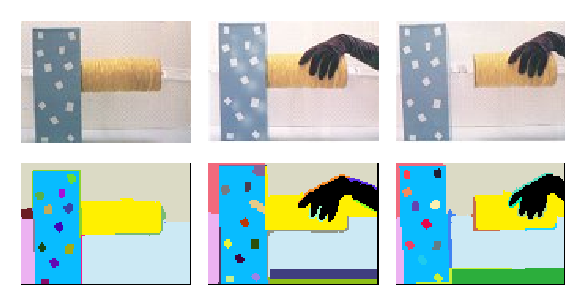
\includegraphics[width=0.5\columnwidth]{fig-pull}}

\caption{
Top: photos of one of Needhan's experiments; a yellow tube is 
pulled away from a blue box with white dots.
Bottom: segmentation of the photos.
}

\label{fig:move-apart}

\end{figure}

In this section we look at experiments that evaluate infant's
expectations about what should move together and what will move
independently; we will compare this to what is technically achievable.
For example, Figure~\ref{fig:move-apart} shows a scenario presented to
infants.



\begin{quote}

It is conceivable that young infants are not exposed to sufficient
contrastive evidence within the context of occlusion events. For
example, infants may seldom observe occlusion events in which: (a) the
objects seen to each side of an occluder either share, or do not
share, the same surface features; and (b) a judgment about the number
of objects present can only be made based on surface features. Without
such evidence, it would be difficult for infants to identify surface
features as important. Even once identified, infants may have few
opportunities to use, and to test, this new knowledge. If surface
features are indeed a less reliable source of information than form
features (e.g. see below), the opportunity to experiment with this new
knowledge might be necessary before infants would be disposed to use
it spontaneously. (Wilcox)

\end{quote}





\subsection{A technical evaluation of Gestalt principles}

How hard is spatiotemporal grouping?
Hard, in the general case.
Of a single, fixated object, while head is not moving much?  and
motion of head is available?

Still tough to do in real time, but the data is there in a form
we could process, given world enough and time.


Motion first -- then shape -- then color/pattern

What is there to learn about shape?  How to see it.

Needham 1999 result is not consistent with the direction of comp
vision research.  Algorithms would group two adjacent objects with
same color-and-pattern but different shapes long before grouping two
adjacent objects with same shape but different color-and-pattern.
Shape is inherently non-local, which color-and-pattern 
can at least to some extent be treated as a local feature.
Computationally, there 
has been little success in recovering shapes in cluttered static scenes.

Why could it make sense?  Lighting variation, color constancy is
really complicated -- maybe better to ignore until had a lot
of experience?

Appearance of surface is subject to a multiplicative effect
with its environment -- shadows, interreflections.

issue of 3D shape, 2D contours.

invariance versus selectivity, classic tradeoff.

If we start with motion, then what we have is motion silhouettes.
We can align the silhouette with the scene, and attempt to train
up methods for predicting the silhouette from the scene.
For a *particular* object at a particular time, it would seem 
best to use all the available correlated features, including 
surface features.  

Why would surface-info not be used in Needham1999 situation,
or be overridden by shape?

Suggest (1) train up generic boundary predictor, so
shape is perceivable, and (2) when shape is available,
segment based on it

Shape information is more important for actually doing things.

(could have more than silhouette from motion of course).


Shape in these particular experiments is maybe not that hard to
recover.

Maybe shape info is easier to use to link motion segmentation
events?  More trustworthy?  Cluster based on shape cues?

For my thesis, with a bunch of segmentations, clusturing by
some course shape measures gave around 88\% accuracy while
clustering by color histogram gave around 99\% accuracy.
But the robot was living in one corner of a lab, with 
relatively constant lighting.  In real life, the story may
be quite different.  Any evidence to suggest this?

Also, the development from grouping anything that moves
together, to then using gaps, is novel and interesting.
Get the cite.




\subsection{Possibilities}

``separately moving'' is not totally clear - consider e.g. a 
jacket, can move arms around a certain amount without body.

Bottom up or top down?  Bottom up and top down?  Interaction
with recognition?

Most commonly, but not always, segmentation is implemented
as a precursor to recognition.  Image comes in, gets
segmented, segments are then run through recognizer.

This is problematic, since segmentation without
recognition is relatively brittle -- it is uninformed.
For something like finding faces, it is more common
not to segment first -- but the common trick here
is to try all possible regions.

Good features, a progression.


\section{INTRO}


Johnson et al re segregation in the presence of partial occlusion.



\noindent General interests:

\begin{itemize}

\item Experiments that demonstrate ``development'' based on experience,
   particularly single or small numbers of episodes

\item Behaviors of the child/robot that have been demonstrated/argued
   to help generate good experience or otherwise help with development.

\end{itemize}


\subsection{Importance of motion?}

We are talking about the {\em development} of perception from an
immature form.  We assume that this development relies on acquiring
some information from the outside world (this isn't necessarily so).
How is this information acquired?  Sensory input is not 
uniformly difficult to interpret -- there are situations in
which it becomes simpler.  One particularly striking case is
the presence of motion.  Coherent group motion of part of the 
scene can be relatively easy to detect, and is a good cue for
the existence and extent of a corresponding object.  
So motion is one good place to start.
%
Moving objects are salient to infants and seem to play an
important role in perceptual learning (BACK THIS UP).
%
In robotics motion has frequently been used in all sorts of
ways.
%
Mention the technical status of motion detection versus
detection of other features (e.g. ``material'').
%
Of course this is by no means the end of the story, there 
are many other features... depth cues etc.

Egomotion is not very useful (relatively speaking).  Movemement of
others or caused by others is useful.  Motion caused by the robot
itself is particularly useful; this could be true of infants but is
moot given the limited motor control available initially.

\subsection{Preamble}

What is perception for?  One classic answer from robotics is that the
goal of perception is to recover, as faithfully as possible, the state
of the world.  That is, some model is made of the world, with some
number of free parameters, and the goal of perception is to find
values for those parameters to bring the model into as close an
alignment as possible with the world.

This view is my no means unquestioned; to achieve a particular
task, the most useful model to estimate may vary.  It may be
trivial, or the robot's behavior may be easier to produce or
describe in alternate ways that don't use the language of
model estimation.

In this paper, we will assume that the robot is engaged
in manipulation tasks (as opposed to, for example, navigation).

{\bf Behavioral view}: strategies that make it likely for the robot
to be looking somewhere useful (hand/eye coordination).
{\bf Model view}: ability to demonstrate flexible knowledge of presence of 
objects and some of their properties.


\subsection{Formalities}

Should provide the clearest possible definition of terms,
as a reference.  Human and robot uses of terms could deviate
from this definition if the deviation is also clearly described.

Object segregation, intermodal integration, object permanence.

Define a cell as the smallest sensing unit, for whichever sensors are
under consideration (e.g. pixels for images).  Assume there are a
fixed number of cells $c_1...c_{N}$.

There is also an unknown set of causes $s_1...s_{M}$, which for a
bounded period of consideration we will consider fixed.  Each cell
$c_i$ provides varying sensor readings $c_i(t)$.  We would like to
generate assignments $a_j(t)$ which, for each cause, lists all the
cells that can reasonably be attributed to that cause.  Then we choose
our causes to be maximally useful in describing the environment.

It is a little difficult to say exactly what judgement should be
made in complicated cases.  Might be better to give examples,
and underspecify.

Specification for object segregation:

$I(t) = [c_1.val(t) ... c_N.val(t)]$

Goal of segregation:
  Find a set $S_i$ = e.g. ${ c_2,c_4,c_5,c_6,... }$ that lists cells that
  belong together at a particular time.
  Find a set of such sets - Z.

Goal of intermodal integration:
  Bring together such sets across modal boundaries.

Goal of object permanence:
  Bring together such sets across time and disappearances.


***********

stuff to be integrated [from Lorenzo]:


The paper focuses on objects. Can we say something about the role of the
body? Achieving eye-hand coordination proved to be extremely useful on the
robots we have worked on. Learning to act is necessary to perform active
exploration of objects (poking/pushing/tapping/grasping). During action the
ability to identify the body helps the robot to focus the attention on the
area of the visual space where "things are happening" (i.e. on the hand upon
contact with the object).


***********

Big potential difference between infants and humans: the role
of manipulation in shaping early perception.  Infants can't
act that much to begin with.





\end{document}


